% REMEMBER: Write the thesis from the view of the reader. How would I like to READ the thesis?
% WHY -> WHAT -> HOW structure

\chapter{Background}%
\label{cha:background}

This chapter will give some background about how Scratch works and why testing Scratch programs is a difficult task.
It will also highlight some previous approaches to automated assessment for Scratch programs.

\section{Scratch}%
\label{sec:scratch}
% Block-based code eliminates the possibility of syntax errors and makes programming more intuitive by letting the user pick blocks from a drawer of pre-defined blocks instead of having the user memorize a programming language's keywords.
% Scratch heavily focuses on multimedia, as graphics and audio can easily be integrated into Scratch projects.
% Whenever a sprite is cloned, it runs all of its scripts, which have a ''when I start as a clone'' hat.

Scratch~\cite{scratch} is a programming language developed by the MIT Media Lab.
Its main goal is to offer an intuitive programming language suited for programming novices and children.
Scratch implements a block-based code system, which eliminates the possibility of syntax errors.
It also allows users to easily integrate graphics and audio into their programs.
Code is run inside a special Scratch VM.
Therefore, Scratch is usually exclusively developed and run through Scratch's web interface, which can be seen in Figure~\ref{fig:scratch_gui}.
\parspace

\begin{figure}[htpb]
    \centering
    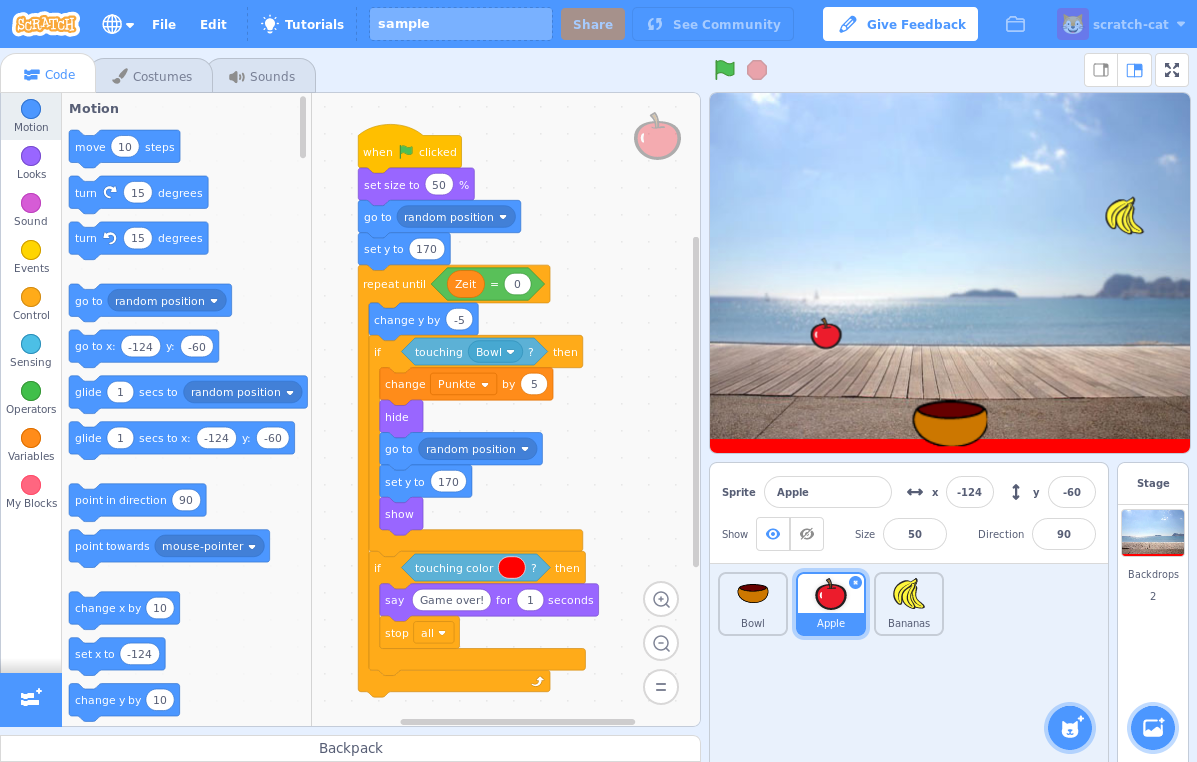
\includegraphics[width=0.75\textwidth]{scratch-gui}
    \caption{A catching game implemented in Scratch}
    \label{fig:scratch_gui}
\end{figure}

\textbf{Code.}
Programming in Scratch is done by sticking together a structure of pre-defined blocks, which are equivalent to statements in traditional programming languages.
Multiple blocks are combined together with a \textit{hat} to make up a \textit{script} (see Figure~\ref{fig:scratch_code}).
Scripts are called through a event, which is defined by their hat.
There are a variety of different events in Scratch.
The main event is the \textit{green flag}, which is the entry point of the program.
This event is emitted when the user starts the program by pressing the start button.
The program then starts by executing all scripts, which are equipped with a ''when green flag is pressed'' hat.
Other events include key presses on the keyboard, clicks on a specific sprite, and events sent from different scripts.
Active scripts effectively run in parallel until the end of each script is reached, or until the script is stopped by itself or another script.
\parspace

\begin{figure}[htpb]
    \centering
    \begin{tikzpicture}
        \node[anchor=south west,inner sep=0] at (0, 0) {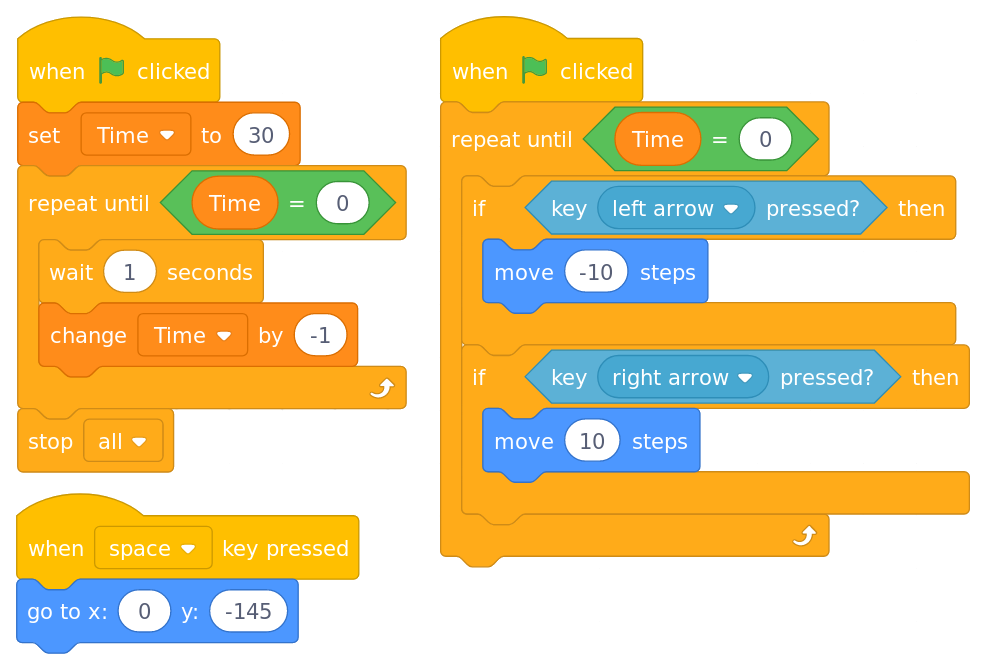
\includegraphics[width=0.6\textwidth]{scratch-code}};
        \draw[red, ultra thick, rounded corners]  (0, 5.27) rectangle (2.20, 6.10);
        \draw[blue, ultra thick, rounded corners] (0, 1.65) rectangle (3.90, 5.10);
        \node[red, font=\large, anchor=north east]   at (0, 6.00) {\texttt{Hat}};
        \node[blue, font=\large, anchor=north east]  at (0, 5.00) {\texttt{Code}};
    \end{tikzpicture}
    \caption{Scratch code}
    \label{fig:scratch_code}
\end{figure}

\textbf{Input and output.}
Scratch programs create interactive two-dimensional animations through a number of visual objects (the \textit{sprites}) on a background (the \textit{stage}).
The program manipulates sprites' appearance, position, size, rotation, visual effects and sounds.
Furthermore, sprites can also display messages and ask the user to type answers into a text box through \texttt{say} and \texttt{ask} blocks.
Programs can react to user input like keyboard key presses, mouse clicks or mouse cursor movement.
Scratch's visual output is rendered in a constant frequency of 30 times per second.
We will call each of the rendered pictures a \textit{frame} and the program execution in between two frames a \textit{step}.
\parspace

\textbf{Sprite and variables.}
Each sprite contains its own scripts and variables.
These variables, as well as the sprite itself can only be manipulated by the sprite's own scripts.
The only exception to this rule is the stage, whose variables are global.
Sprites can communicate with each other through a messaging system and through the stage's variables.
By \textit{cloning} sprites, the program can create multiple instances of a sprite, which behave alike.
The cloned sprites then also share the original sprite's variables.

\section{Previous Testing Approaches}%
\label{sec:previous_testing_approaches}

Although automatic assessment of Scratch programs is still an open problem,
at least two other projects have tackled this task through different approaches.
\parspace

\textbf{Hairball.}
Boe et al. developed Hairball~\cite{hairball} to perform static analysis on Scratch programs.
Hairball is implemented as a standalone Python program.
It allows users to load a saved project file and analyze it by iterating through its blocks.
% Example applications of Hairball are detecting code smells or finding out if a desired programming concept is implemented in the program.
A example application of this program is the web-based assessment tool called Dr. Scratch~\cite{drscratch} by Jes\'{u}s et al..
Dr. Scratch uses Hairball to measure the complexity of uploaded Scratch programs in various categories and scores them accordingly.
Though Hairball is very useful for analyzing programs statically, testing the functionality of a program with it would be very difficult.
In order to do this, a dynamic testing approach is more suitable, because it can simply observe to programs behaviour instead of having to deduct it from the programs source code.
\parspace

\textbf{ITCH.}
ITCH (Individual Testing of Computer Homework for Scratch Assignments)~\cite{itch} by David E. Johnson is another Scratch assessment tool.
Like Hairball, it is also implemented in Python.
But it follows an entirely different approach.
ITCH performs functional testing on Scratch programs, which have their functionality reduced to simple textual input and output operations.
Scratch supports these operations through "ask" and "say" blocks.
In order to automate the input and output, ITCH replaces these blocks with structures, which give the program configured input text, and save the resulting output to the project file.
ITCH then executes the program, saves it, and analyzes the saved project file to generate a test report.
This allows simple input-output-testing for Scratch, which is useful for testing the correctness of an implemented algorithm.
But ITCH has a major drawback: Reducing Scratch programs to textual IO means, that only a small subset of Scratch's functionality is available to the programs under test.
Sprite manipulation and such cannot be tested with ITCH.
If the only reason to adopt Scratch is its block-based code system, there exist other block-based programming environments, that serve as a front-end to more common programming languages, which can be tested more easily.
An example for this is BlockPy~\cite{blockpy}, which translates its block-based code into Python.

% \section{Black Box Testing}
%
% - Black box approach:
%     - Block box testing bases tests on the specification of the tested program
%     - Tests are written without knowledge of the internals of a program
%     - Program is seen as a ''black box'' that takes some input and produces some output.
%     - Program specification is in the case of Scratch programs most likely a task description for some course or tutorial
%
%     - Input for the black box is user interaction through mouse and keyboard
%     - Interact only how a user can interact with the program
%         - Since Scratch can only be controlled through user interaction and has no API to call blocks or scripts,
%           it only makes sense to control the program this way in the test
%         - No information about the internals of the program other than sprite and variable names
%             - Sprite names should be included in the specification so the test can more easily identify sprites
%             - Giving no or little information about the implementation makes sense for a task description
%     - Output of the black box are changes on Scratch's stage
%     - Test only what the user sees
%         - Only information about sprites and variables (both can be shown on screen)
%         - Sprite positions, movement, looks, etc.

\section{Challenges of Testing Scratch Programs}
\label{sec:challenges_of_testing_scratch_programs}

Dynamically testing Scratch programs is not a straightforward task.
There exist multiple challenges, that have to be overcome in order to test Scratch programs accurately.
This section will go over these challenges and explain each one of them.
% TODO: This section explains these challenges and how the presented approach overcomes them.
\parspace

\textbf{Scratch's code system.}
Scratch does not have a traditional mechanism to structure code into methods, which return values.
Unit test cases usually call methods with some input and check the returned value, but this is not possible in Scratch.
Additionally, scripts run in parallel and may depend on one another.
This makes it hard to test a part of the program in isolation from the rest of the program.
One could circumvent this problem by restricting the tested programs, like ITCH~\cite{itch} does it,
but that defeats the purpose of using Scratch as a language.
% To deal with this challenge, this work proposes a black-box testing approach.
% This way, the test code does not have to concern itself with the internals of the program.
% Scratch programs can be controlled by simulating user input, instead of calling specific scripts.
% Tests can then check the visual and auditory output of the program.
\parspace

\textbf{GUI input and output.}
Scratch is entirely run inside a graphical user interface and therefore lacks traditional IO mechanisms.
Its output consists of visual animations and audio, which are difficult to analyze automatically.
Likewise, Scratch's input, which mainly consists of keyboard and mouse input, can make interacting with the program problematic.
% We are going to deal with this problem by creating a wrapper around Scratch,
% which can be used to simulate input and access information about the sprites which make up the output.
% Tests can then use methods, which the wrapper provides, instead of manually interacting with the Scratch program.
\parspace

\textbf{Randomness.}
Scratch provides blocks to incorporate randomness into programs.
Non-determinism is problematic for testing in general and not just for Scratch,
but Scratch programs tend to often make use of randomness,
since it can make game-like programs more interesting.
This is especially relevant in the context of automated grading.
Programming tasks for students in conventional programming languages are usually deterministic.
However, Scratch assignments may tend to feature randomness to make the task more exciting.
\parspace

\textbf{Missing Initialization.}
Scratch programs don't start with a fixed configuration of sprites and variables.
When the program is loaded, it loads the sprite attributes and variable values from the project file and restores that state.
Then, when the program is run, it starts with this state, but subsequent executions of the program continue with the configuration,
which the last run of the program left after it ended.
Scratch programs can deal with this by doing initialization in the beginning, but many don't.
Therefore, if a program is run multiple times for testing, the initial sprite and variable configuration needs to be restored.
\parspace

\textbf{Fuzziness of properties.}
Scratch programs often don't deal with exact values,
since small differences in sprite properties are generally indistinguishable in the program's output.
This can make testing more difficult, since assertions have to take small deviations into consideration.
Scratch itself also makes dealing with exact values unattractive.
In the Scratch GUI, sprites can initially be positioned on the stage via drag and drop.
Also, instead of comparing exact positions, Scratch offers built in blocks to directly check for sprite collisions.
\parspace

\textbf{Tracking of properties.}
In order to test movement or animations, we need to track sprite information over a period of time.
Hence, we need a way to periodically access sprite attributes (and variables) during the program execution.
\parspace
